% -----------------------
\subsection{Pfeilspitzen}
% -----------------------
\begin{minipage}{0.7\textwidth}
  \footnotesize
  \input{arrowright.code}
\end{minipage}\hfill
\begin{minipage}{0.29\textwidth}
  \centering
  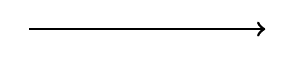
\begin{tikzpicture}[line width=1pt]
    % Pfeilspitze rechts
    \draw[->] (0, 0) -- (3, 0);
  \end{tikzpicture}
\end{minipage}

\begin{minipage}{0.7\textwidth}
  \footnotesize
  \input{arrowleft.code}
\end{minipage}\hfill
\begin{minipage}{0.29\textwidth}
  \centering
  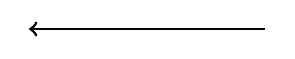
\begin{tikzpicture}[line width=1pt]
    % Pfeilspitze links
    \draw[<-] (0, 0) -- (3, 0);
  \end{tikzpicture}
\end{minipage}

\begin{minipage}{0.7\textwidth}
  \footnotesize
  \input{arrowleftright.code}
\end{minipage}\hfill
\begin{minipage}{0.29\textwidth}
  \centering
  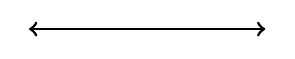
\begin{tikzpicture}[line width=1pt]
    % Pfeilspitzen links und rechts
    \draw[<->] (0, 0) -- (3, 0);
  \end{tikzpicture}
\end{minipage}

\begin{minipage}{0.7\textwidth}
  \footnotesize
  \input{arrowdouble.code}
\end{minipage}\hfill
\begin{minipage}{0.29\textwidth}
  \centering
  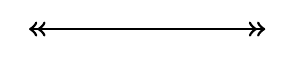
\begin{tikzpicture}[line width=1pt]
    % doppelte Spitze
    \draw[<<->>] (0, 0) -- (3, 0);
  \end{tikzpicture}
\end{minipage}

\begin{minipage}{0.7\textwidth}
  \footnotesize
  \input{arrowpipeonly.code}
\end{minipage}\hfill
\begin{minipage}{0.29\textwidth}
  \centering
  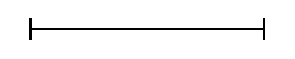
\begin{tikzpicture}[line width=1pt]
    % stumpfe Enden
    \draw[|-|] (0, 0) -- (3, 0);
  \end{tikzpicture}
\end{minipage}

\begin{minipage}{0.7\textwidth}
  \footnotesize
  \input{arrowpipe.code}
\end{minipage}\hfill
\begin{minipage}{0.29\textwidth}
  \centering
  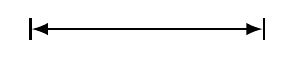
\begin{tikzpicture}[line width=1pt]
    % Spitze mit Begrenzung
    \draw[|<->|, >=latex] (0, 0) -- (3, 0);
  \end{tikzpicture}
\end{minipage}

\begin{minipage}{0.7\textwidth}
  \footnotesize
  \input{arrowlatex.code}
\end{minipage}\hfill
\begin{minipage}{0.29\textwidth}
  \centering
  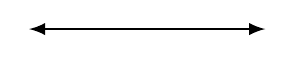
\begin{tikzpicture}[line width=1pt]
    % Form: latex
    \draw[<->, >=latex] (0, 0) -- (3, 0);
  \end{tikzpicture}
\end{minipage}

\begin{minipage}{0.7\textwidth}
  \footnotesize
  \input{arrowstealth.code}
\end{minipage}\hfill
\begin{minipage}{0.29\textwidth}
  \centering
  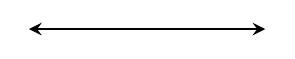
\begin{tikzpicture}[line width=1pt]
    % Form: stealth
    \draw[<->, >=stealth] (0, 0) -- (3, 0);
  \end{tikzpicture}
\end{minipage}

\begin{minipage}{0.7\textwidth}
  \footnotesize
  \input{arrowtoreversed.code}
\end{minipage}\hfill
\begin{minipage}{0.29\textwidth}
  \centering
  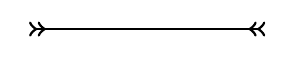
\begin{tikzpicture}[line width=1pt]
    % doppelte Spitze: to reversed
    \draw[<<->>, >=to reversed] (0, 0) -- (3, 0);
  \end{tikzpicture}
\end{minipage}

\begin{minipage}{0.7\textwidth}
  \footnotesize
  \input{arrowstealthreversed.code}
\end{minipage}\hfill
\begin{minipage}{0.29\textwidth}
  \centering
  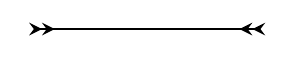
\begin{tikzpicture}[line width=1pt]
    % doppelte Spitze: stealth reversed
    \draw[<<->>, >=stealth reversed] (0, 0) -- (3, 0);
  \end{tikzpicture}
\end{minipage}

\begin{minipage}{0.7\textwidth}
  \footnotesize
  \input{arrowcircle.code}
\end{minipage}\hfill
\begin{minipage}{0.29\textwidth}
  \centering
  \begin{tikzpicture}[line width=1pt]
    % runde Enden
    % benoetigt \usetikzlibrary{arrows}
    \draw[o-o] (0, 0) -- (3, 0);
  \end{tikzpicture}
\end{minipage}

\begin{minipage}{0.7\textwidth}
  \footnotesize
  \input{arrowparenthesis.code}
\end{minipage}\hfill
\begin{minipage}{0.29\textwidth}
  \centering
  \begin{tikzpicture}[line width=1pt]
    % abgerundete Spitzen
    % benoetigt \usetikzlibrary{arrows}
    \draw[(-)] (0, 0) -- (3, 0);
  \end{tikzpicture}
\end{minipage}

\begin{minipage}{0.7\textwidth}
  \footnotesize
  \input{arrowbrackets.code}
\end{minipage}\hfill
\begin{minipage}{0.29\textwidth}
  \centering
  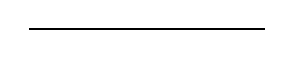
\begin{tikzpicture}[line width=1pt]
    % eckige Spitzen
    % benoetigt \usetikzlibrary{arrows}
    \draw[[-{]}] (0, 0) -- (3, 0);
  \end{tikzpicture}
\end{minipage}

\begin{minipage}{0.7\textwidth}
  \footnotesize
  \input{arrowdiamond.code}
\end{minipage}\hfill
\begin{minipage}{0.29\textwidth}
  \centering
  \begin{tikzpicture}[line width=1pt]
    % Form: diamond
    % benoetigt \usetikzlibrary{arrows}
    \draw[<->, >=diamond] (0, 0) -- (3, 0);
  \end{tikzpicture}
\end{minipage}

